\section{Fiber Orientation Optimization}

\indent

CFRPs exhibit maximum strength when fibers align appropriately with the loads. Therefore, fiber orientation within parts is critical. Finite element analysis software will be utilized to determine optimal fiber orientation and printing tool paths will be generated from this data.

\subsection{Finite Element Analysis}

\indent

\emph{ANSYS} finite element software will be used to determine fiber orientation within printed parts. The \emph{Composite PrepPost} package, which is specifically designed to assess the strength of composite structures, will be used. The package utilizes shell elements that contain matrix and fiber material properties. The software also contains multiple laminate failure criteria and can perform optimization loops to determine the strongest configuration of fiber angles. For instance, a tube can discretized into a number of shell elements, assigned a number of layers, given isotropic matrix material properties and orthotropic fiber material properties, and iterated through different fiber angles to calculate stress and deformation gradients across the entire part (at all angles or at only the strongest angle). Therefore, once the specific printed part geometry for the curved layer carbon fiber is determined, this software will be used to find optimal fiber orientation(s).\footnote{Dr. Wootton has advised that many computation analyses usually overshoot experimental strength results. However, experimental and theoretical results will typically agree in trends and the computational model will sufficiently locate the weakest area(s) of the geometry.}\\

\subsubsection{ACP Results}

%% Deformation

\begin{figure}[htp]
\centering
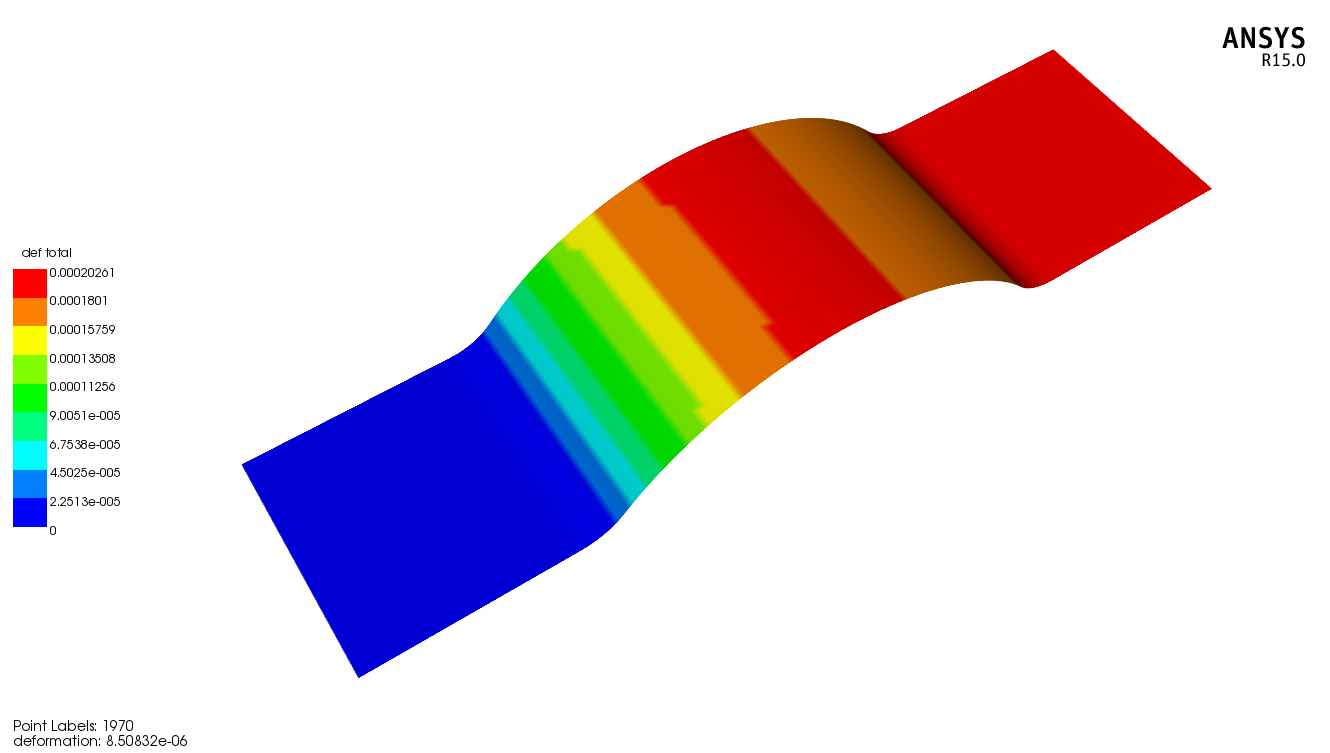
\includegraphics[width=1\textwidth]{./figures/fea/fea-acp-tot-def}
\caption{Total displacement FEA result.}
\label{fig:fea-acp-tot-def}
\end{figure}

\begin{figure}[htp]
\centering
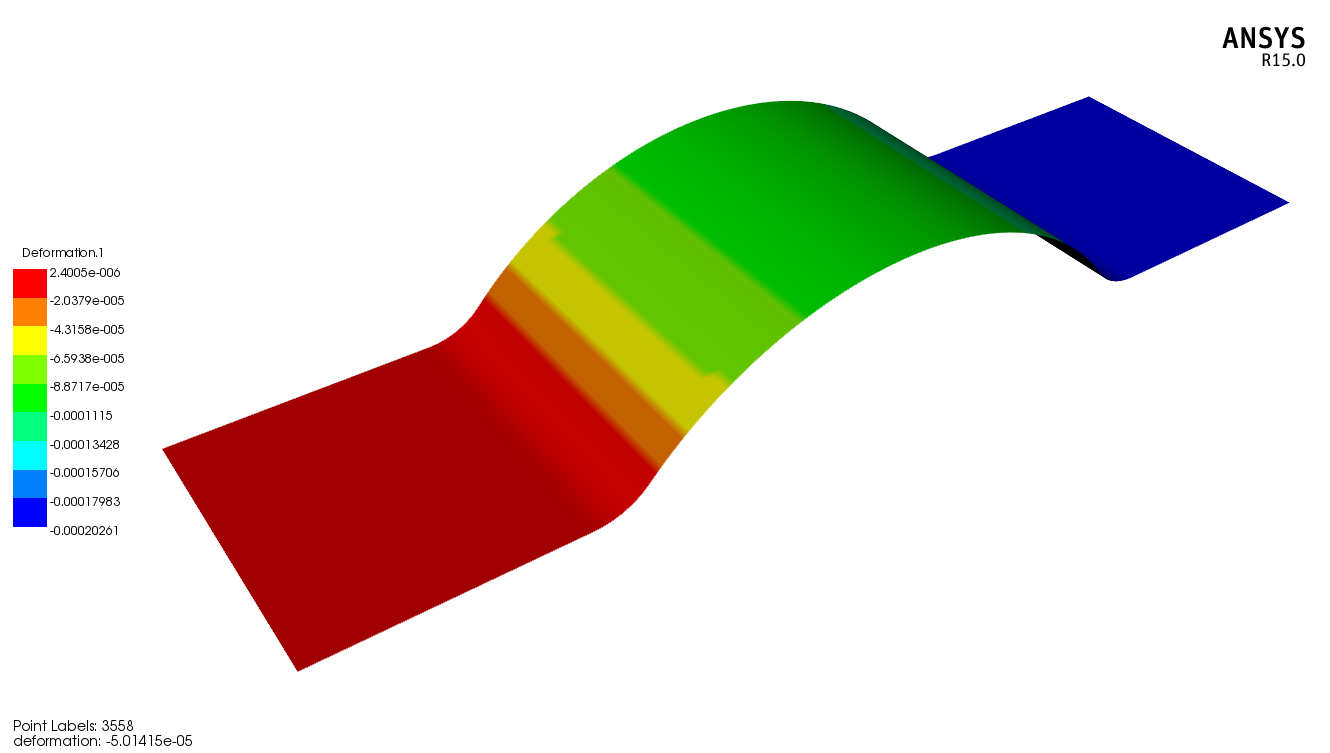
\includegraphics[width=1\textwidth]{./figures/fea/fea-acp-x-def}
\caption{X direction displacement FEA result.}
\label{fig:fea-acp-x-def}
\end{figure}

\begin{figure}[htp]
\centering
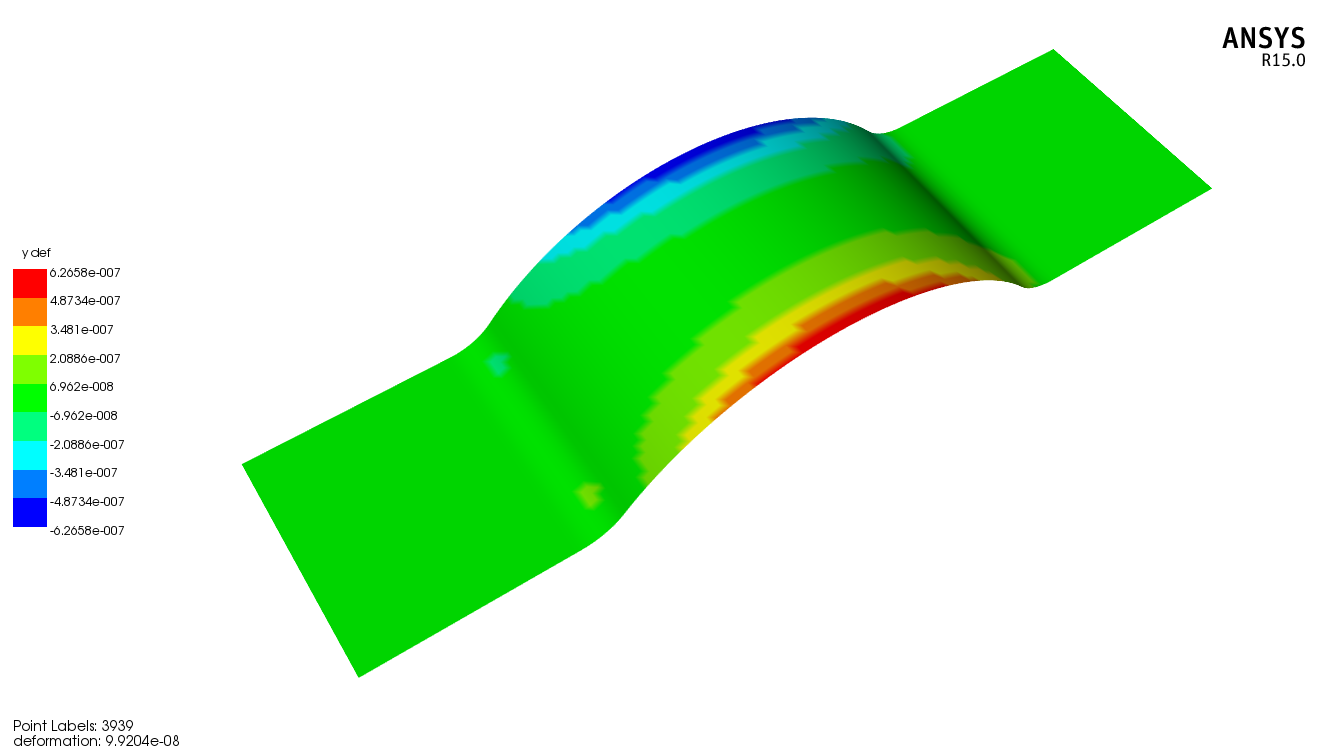
\includegraphics[width=1\textwidth]{./figures/fea/fea-acp-y-def}
\caption{Y direction displacement FEA result.}
\label{fig:fea-acp-y-def}
\end{figure}

\begin{figure}[htp]
\centering
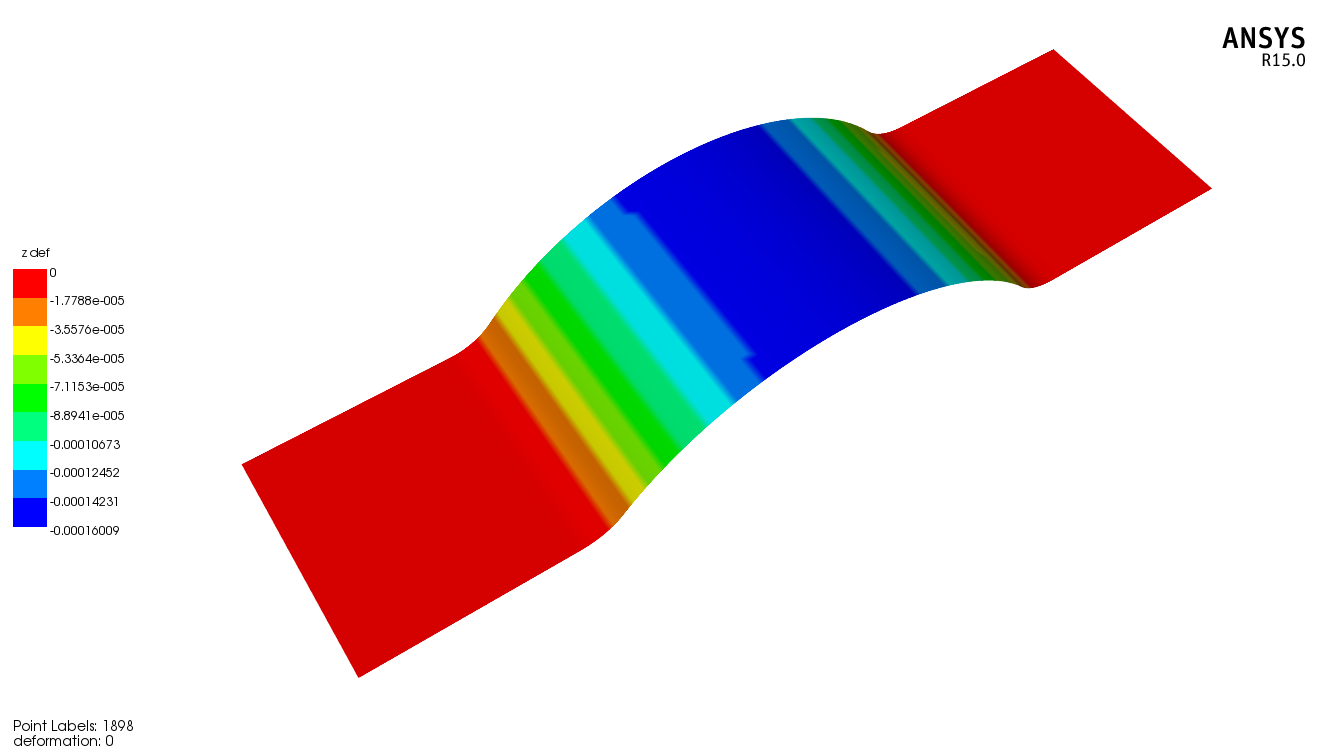
\includegraphics[width=1\textwidth]{./figures/fea/fea-acp-z-def}
\caption{Mesh overview of the composite model in \textit{ACP} with a solid-body display state applied.}
\label{fig:fea-acp-z-def}
\end{figure}

%%% Puck Failure Results

\begin{figure}[htp]
\centering
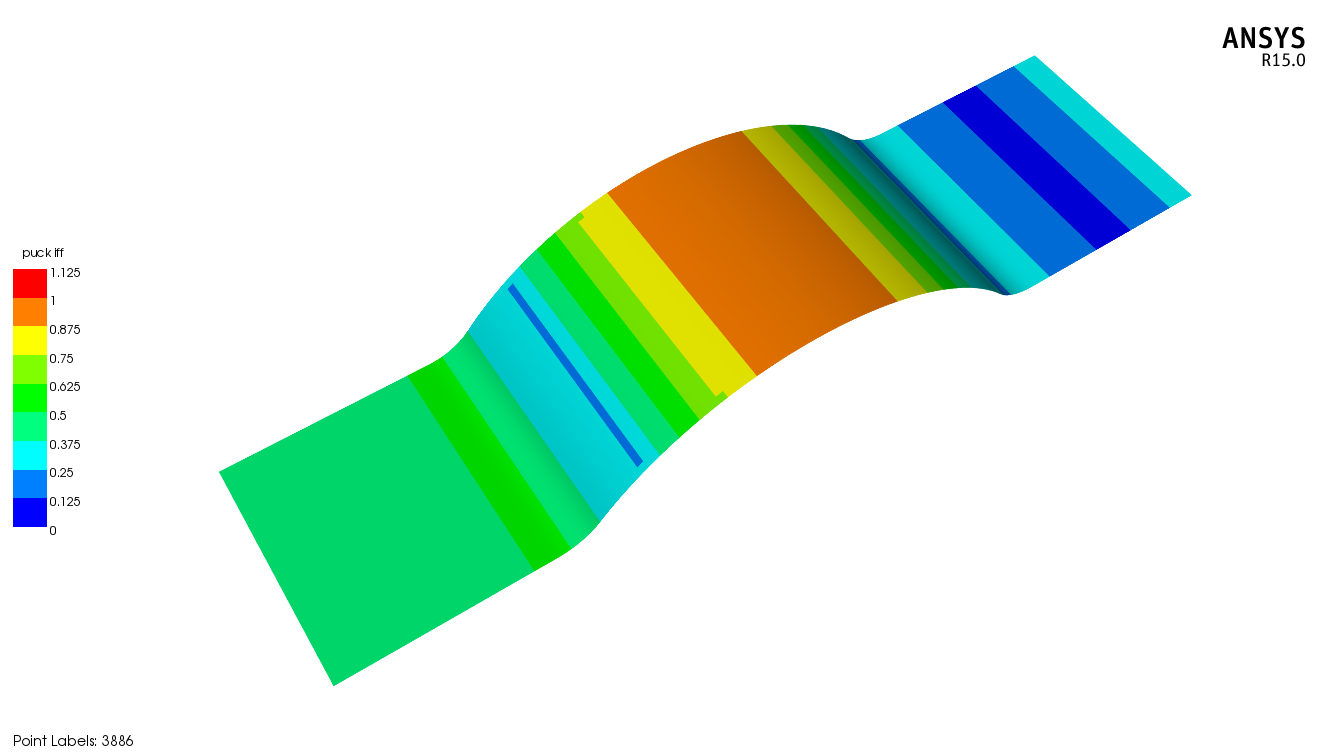
\includegraphics[width=1\textwidth]{./figures/fea/fea-acp-pfailure-notext}
\caption{Puck Failure contour plot.}
\label{fig:fea-acp-pfailure-notext}
\end{figure}

\begin{figure}[htp]
\centering
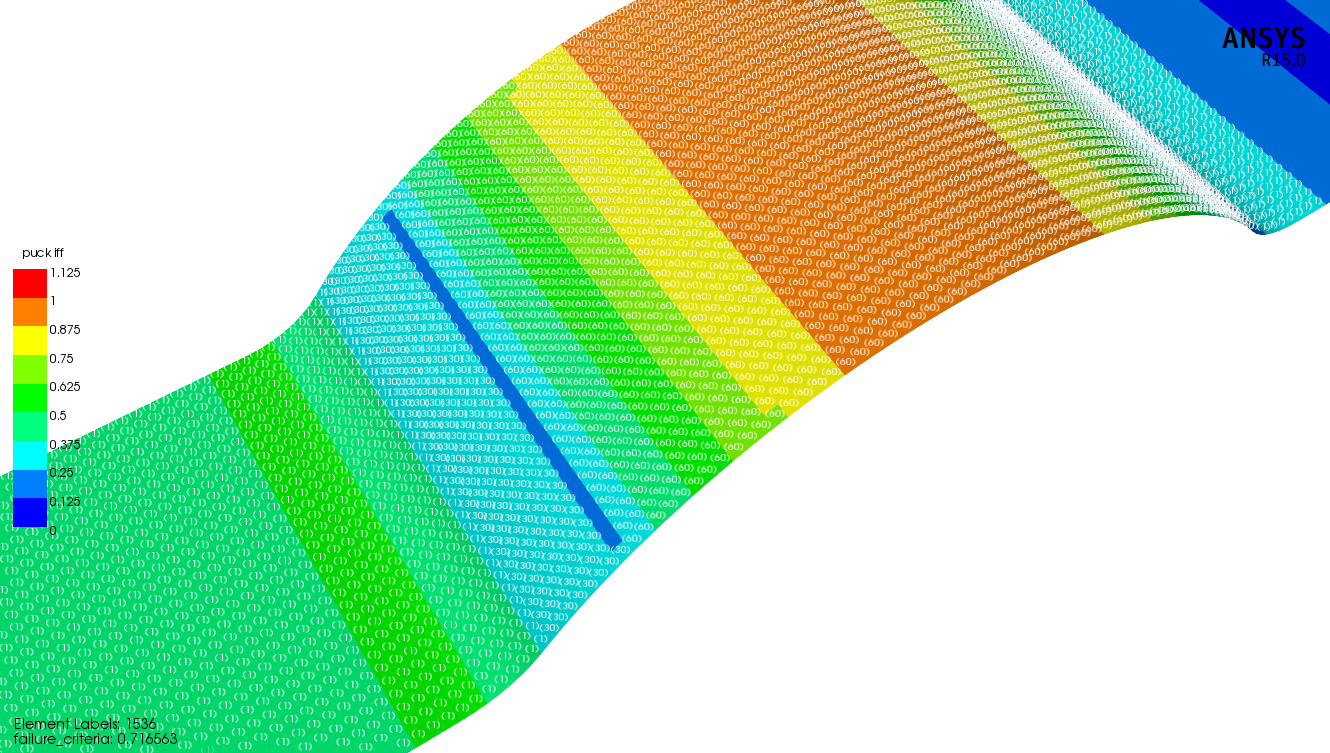
\includegraphics[width=1\textwidth]{./figures/fea/fea-acp-pfailure-layer-closeup}
\caption{Closeup of Puck Failure contour plot with tabulated failing layer.}
\label{fig:fea-acp-pfailure-layer-closeup}
\end{figure}

\begin{figure}[htp]
\centering
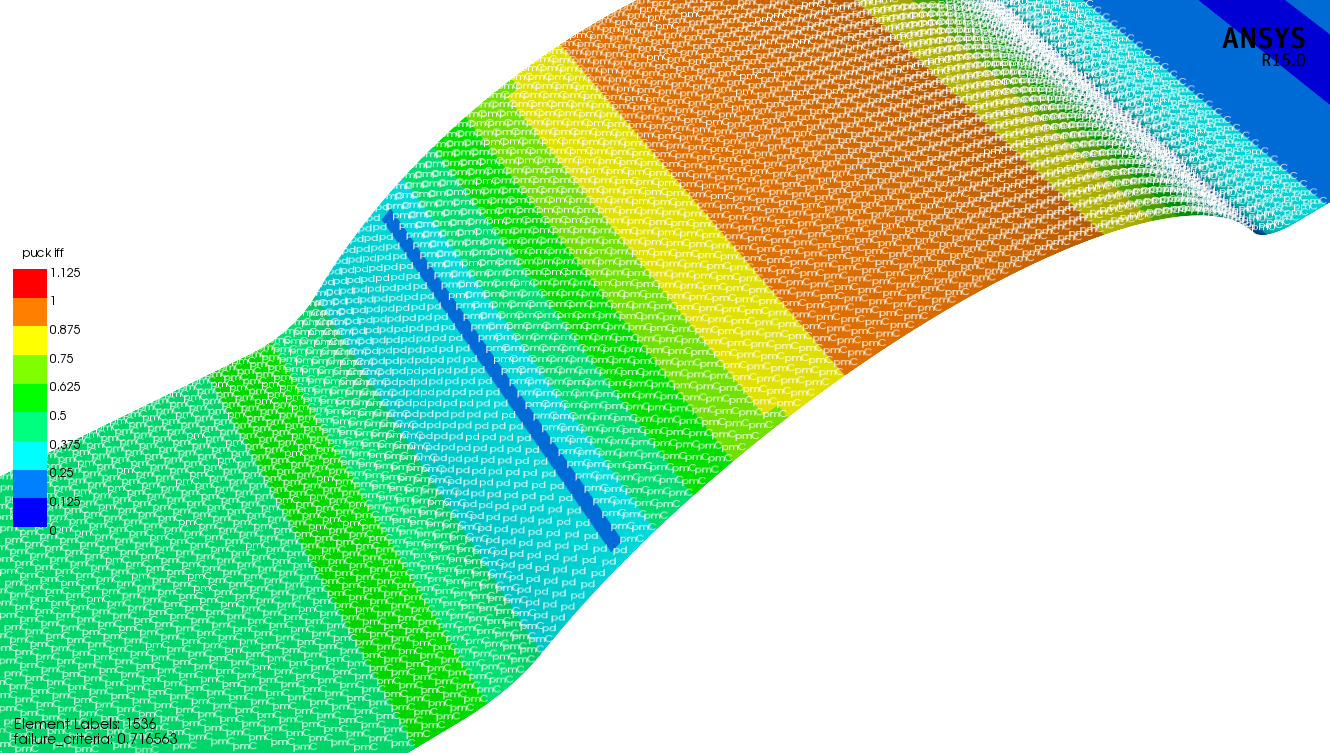
\includegraphics[width=1\textwidth]{./figures/fea/fea-acp-pfailure-mode-closeup}
\caption{Closeup of Puck Failure contour plot with tabulated failure modes.}
\label{fig:fea-acp-pfailure-mode-closeup}
\end{figure}

\clearpage

\subsubsection{Comparison to Puck Failure Criterion}

\clearpage

\subsection{Toolpath Generation}

\indent

The toolpath for an FDM 3D printer is the path in space that the extruder follows while it prints a part. In most FDM printers, the toolpath is sent to the machine in a machine control language known as Gcode. Many existing programs, open source and proprietary, can be used to turn an STL file into Gcode. Because current 3D printers all use flat layers, these slicing programs are not suitable for creating curved-layer toolpaths. Fortunately, parts of some modular open source slicing programs may be repurposed for generating curved layer toolpaths. Once the toolpaths are generated, they will be converted to TP (FANUC's robot control language) and sent to the FANUC robot controller. \\
